\documentclass[12pt, a4paper]{article}

% Pacotes essenciais para português e formatação
\usepackage[utf8]{inputenc}
\usepackage[T1]{fontenc}
\usepackage[portuguese]{babel}
\usepackage{graphicx} 
\usepackage{hyperref} 
\usepackage{geometry}
\usepackage{float} 
\geometry{a4paper, top=3cm, bottom=2cm, left=3cm, right=2cm}

\title{\textbf{Documentação do Sistema: Academia Fit}}
\author{Guilherme Matos(GU3054179) \\
    Fabio Baptista(GU3055302)\\
    Isaque Gonçalves(GU3055515)}
\date{2 de Julho de 2026}

\begin{document}

% Capa e Sumário
\maketitle
\tableofcontents
\newpage

\section{Objetivo do Sistema}
O Sistema Academia Fit tem como objetivo automatizar e gerenciar as operações essenciais de uma academia, oferecendo um portal web responsivo e unificado para alunos, instrutores (funcionários) e gerentes. A plataforma visa facilitar desde o cadastro e autenticação segura de usuários até o acompanhamento de treinos diários, gestão de fichas de exercícios e controle em tempo real dos níveis de acesso corporativo.

\section{Equipe e Funções}
\begin{itemize}
    \item \textbf{Guilherme:} (Documentação, Front-End)
    \item \textbf{Isaque:} (Back-End, Front-End)
    \item \textbf{Fabio:} (Back-End, Front-End)
\end{itemize}

\section{Requisitos do Sistema}

\subsection{Requisitos Funcionais (RF)}
\begin{itemize}
    \item \textbf{RF01 - Gestão de Autenticação:} O sistema deve permitir o cadastro de novos usuários, criptografando a senha em SHA-256 e mantendo a conta inativa até a validação via token enviado por e-mail (integração com Mailtrap).
    \item \textbf{RF02 - Controle de Acesso (Autorização):} O sistema deve controlar o acesso às rotas privadas através de um \textit{Filter} (AuthFilter), validando a sessão ativa e o nível de permissão (Aluno, Funcionário ou Gerente) para cada URI requisitada.
    \item \textbf{RF03 - Recuperação de Credenciais:} O sistema deve prover um fluxo de recuperação de senha gerando um UUID temporário, enviado por e-mail, permitindo a alteração segura da senha através de requisições assíncronas.
    \item \textbf{RF04 - Painel do Aluno (Check-in):} Usuários com a \textit{role} ``ALUNO'' devem visualizar seus blocos de treino (A, B, C) e registrar a presença (check-in) diária no sistema.
    \item \textbf{RF05 - Painel do Instrutor (Prescrição de Treinos):} Usuários com a \textit{role} ``FUNCIONARIO'' devem ser capazes de criar e editar estruturas de blocos de exercícios, bem como vincular dinamicamente esses treinos ao CPF dos alunos matriculados.
    \item \textbf{RF06 - Painel Administrativo (Gerência):} Usuários com a \textit{role} ``GERENTE'' devem ter acesso a uma interface de controle em tempo real para alterar o nível de acesso (Role-Based Access Control - RBAC) dos usuários cadastrados no sistema.
\end{itemize}

\subsection{Requisitos Não Funcionais (RNF)}
\begin{itemize}
    \item \textbf{RNF01 - Plataforma e Linguagem:} A aplicação deve ser construída na plataforma Jakarta EE (Servlets e JSP), utilizando a linguagem Java (versão 21) e empacotada via Apache Maven.
    \item \textbf{RNF02 - Servidor de Aplicação:} O sistema deve ser implantado e executado no servidor web Apache Tomcat versão 11.0.
    \item \textbf{RNF03 - Persistência de Dados:} O armazenamento de dados relacionais deve ser feito no banco de dados MySQL Server 8.4, utilizando o driver \texttt{mysql-connector-j}.
    \item \textbf{RNF04 - Comunicação Cliente-Servidor:} As interfaces devem se comunicar com o back-end exclusivamente via requisições AJAX utilizando a biblioteca jQuery 3.7.1, trafegando os dados no formato JSON (serializados via biblioteca Gson 2.14.0).
    \item \textbf{RNF05 - Interface de Usuário (UI):} O front-end deve ser responsivo, construído com HTML5, CSS3, e o framework Bootstrap 5.3.3, integrando a biblioteca FontAwesome 6.4.0 para iconografia.
\end{itemize}

\section{Diagramas}

\subsection{Diagrama de Casos de Uso}
O diagrama a seguir ilustra as interações dos atores (Aluno, Funcionário e Gerente) com as principais funcionalidades do sistema.
\begin{figure}[H]
    \centering
    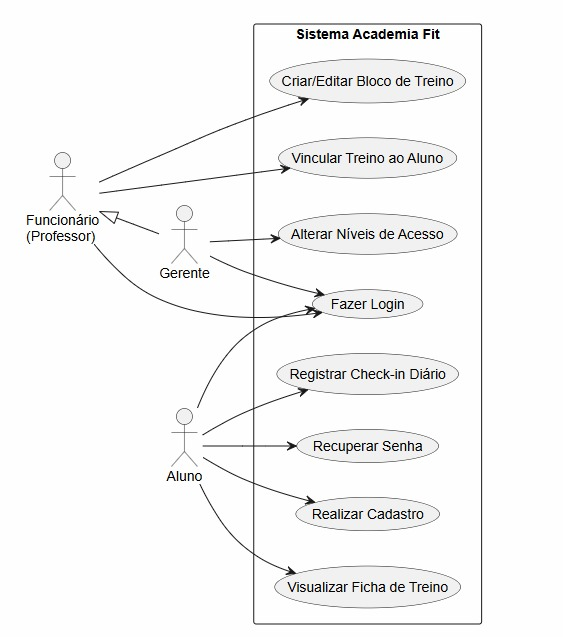
\includegraphics[width=0.7\textwidth]{imagens/Casos_De_Uso.jpg}
    \caption{Diagrama de Casos de Uso}
\end{figure}

\subsection{Diagrama de Classes}
Este diagrama apresenta a estrutura estática do sistema, destacando os modelos de dados, seus atributos, métodos e os relacionamentos de herança e composição.
\begin{figure}[H]
    \centering
    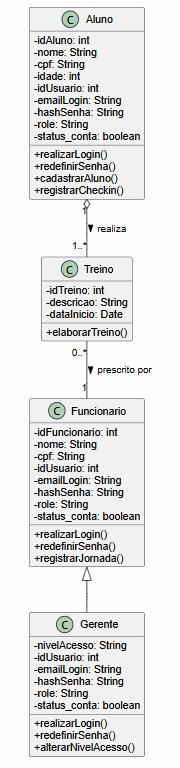
\includegraphics[width=0.3\textwidth]{imagens/Classes.png}
    \caption{Diagrama de Classes}
\end{figure}

\subsection{Diagrama Entidade-Relacionamento (ERD)}
O ERD abaixo detalha a modelagem física do banco de dados MySQL, evidenciando as chaves primárias (PK), chaves estrangeiras (FK) e as cardinalidades entre as tabelas.
\begin{figure}[H]
    \centering
    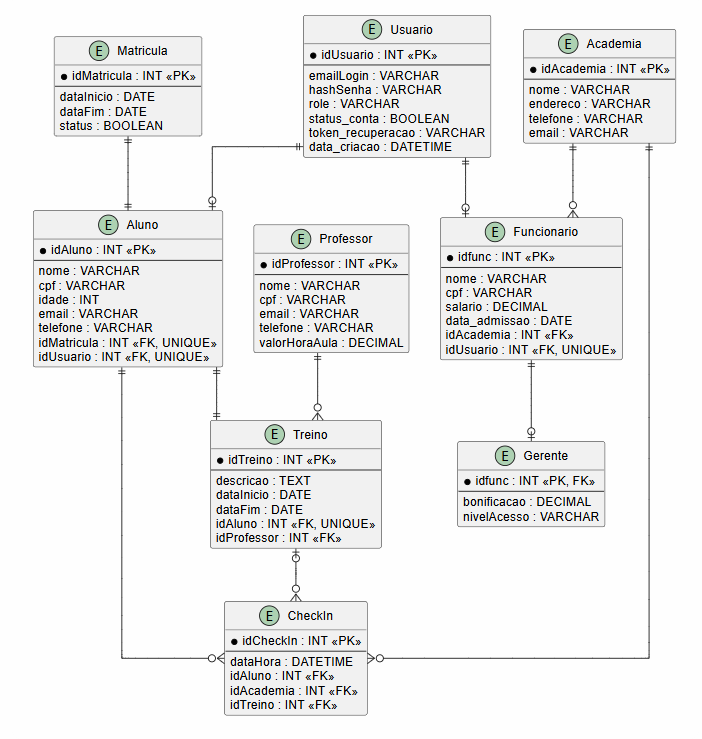
\includegraphics[width=0.8\textwidth]{imagens/ERD.png}
    \caption{Diagrama Entidade-Relacionamento (ERD)}
\end{figure}

\subsection{Diagramas de Sequência}
Esta seção detalha o fluxo de mensagens e a ordem de execução no tempo para os principais processos de negócio do sistema.

\subsubsection{Fluxo do Gerente (RBAC)}
\begin{figure}[H]
    \centering
    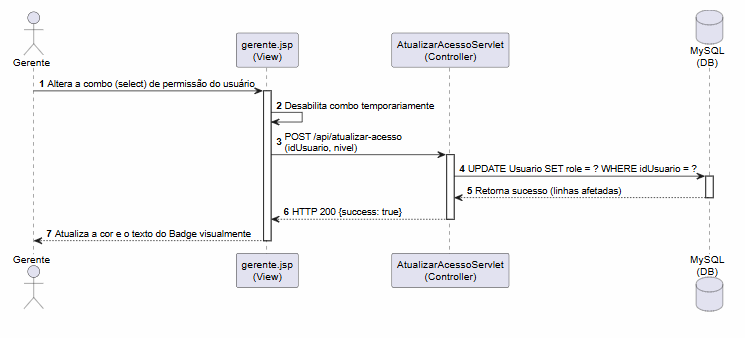
\includegraphics[width=0.95\textwidth]{imagens/Sequencia_Gerente.png}
    \caption{Diagrama de Sequência - Alteração de Nível de Acesso}
\end{figure}

\subsubsection{Fluxo do Professor (Vincular Treino)}
\begin{figure}[H]
    \centering
    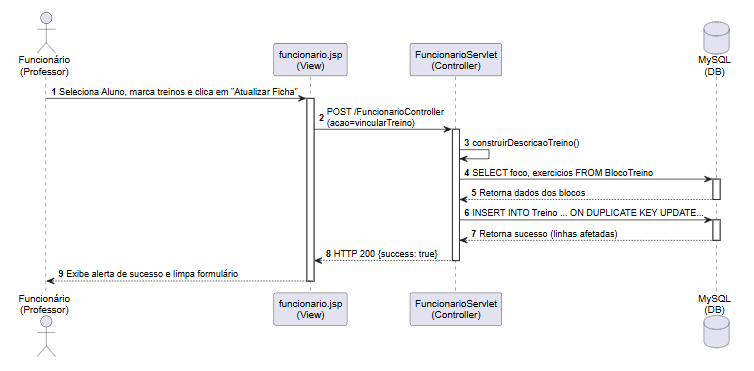
\includegraphics[width=0.95\textwidth]{imagens/Sequencia_Professor.png}
    \caption{Diagrama de Sequência - Prescrição e Vinculação de Treino}
\end{figure}

\subsubsection{Fluxo do Aluno (Check-In)}
\begin{figure}[H]
    \centering
    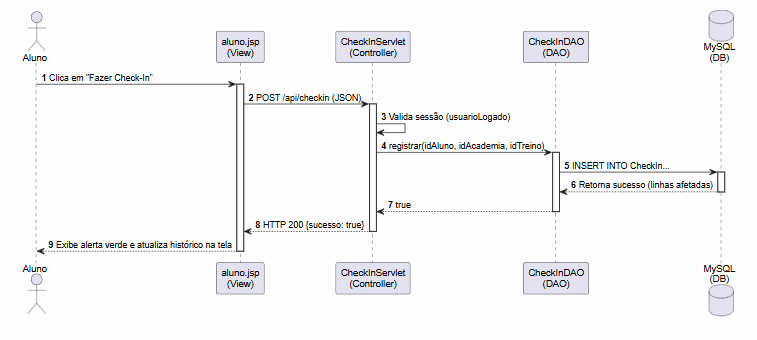
\includegraphics[width=0.95\textwidth]{imagens/Sequencia_Aluno.png}
    \caption{Diagrama de Sequência - Registro de Presença (Check-In)}
\end{figure}

\subsubsection{Fluxo de Autenticação (Login)}
\begin{figure}[H]
    \centering
    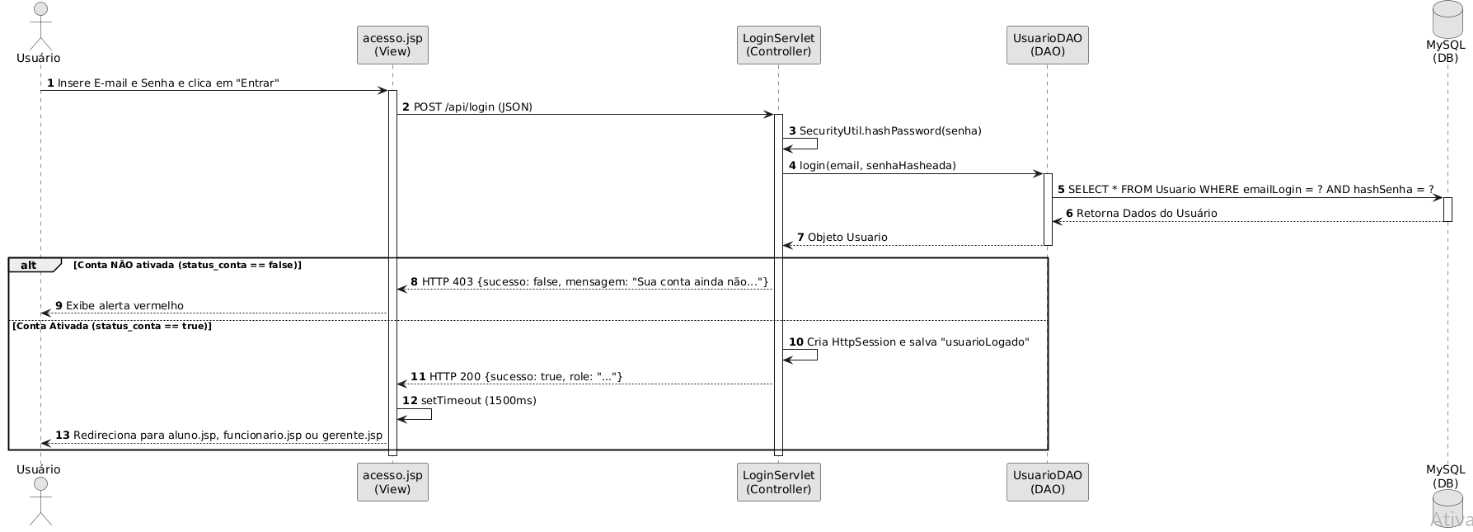
\includegraphics[width=0.95\textwidth]{imagens/Sequencia_Login.png}
    \caption{Diagrama de Sequência - Login e Controle de Sessão}
\end{figure}

\subsubsection{Fluxo de Recuperação de Senha}
\begin{figure}[H]
    \centering
    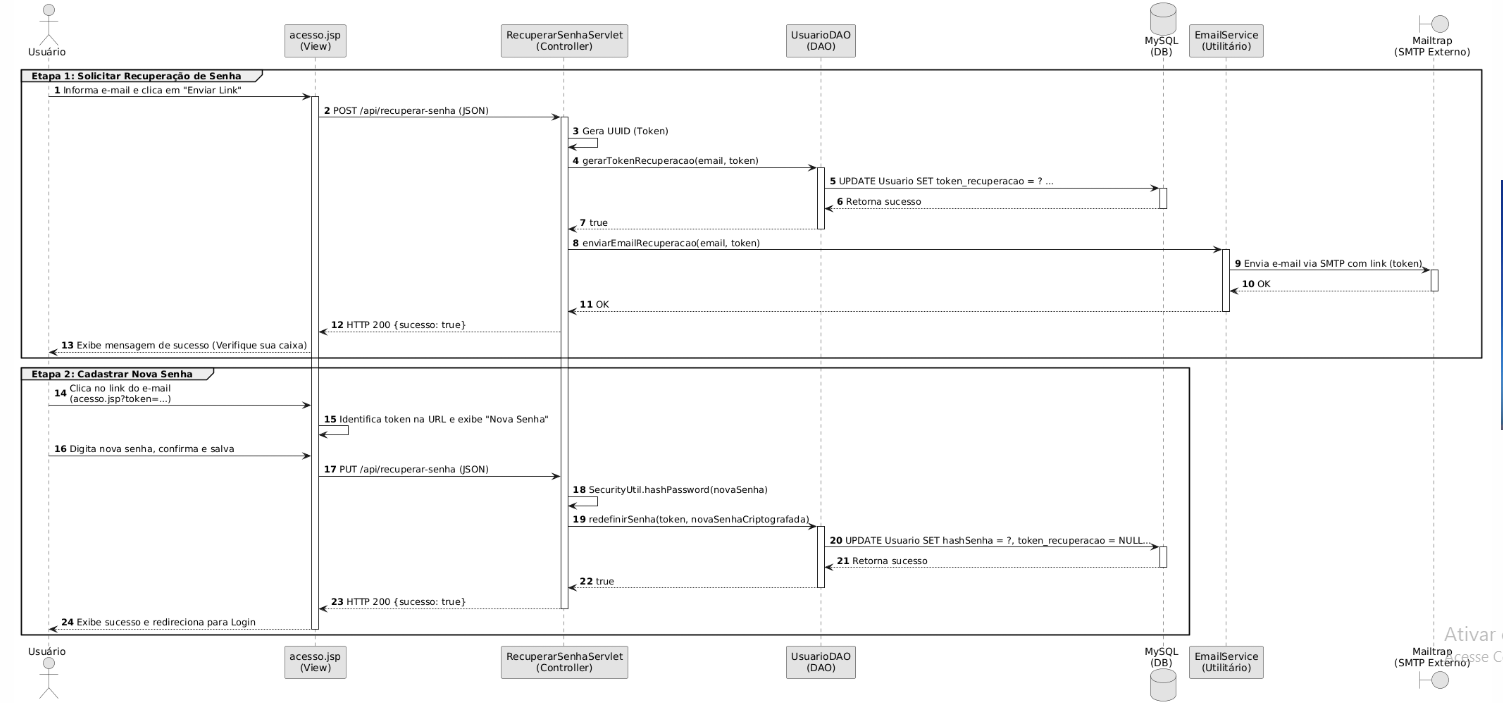
\includegraphics[width=0.95\textwidth]{imagens/Sequencia_Recuperar.png}
    \caption{Diagrama de Sequência - Recuperação de Senha}
\end{figure}

\subsubsection{Fluxo de Cadastro via Mailtrap}
\begin{figure}[H]
    \centering
    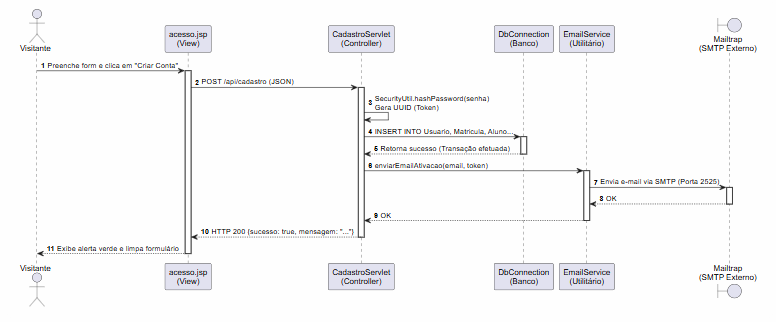
\includegraphics[width=0.95\textwidth]{imagens/Sequencia_Mailtrap.png}
    \caption{Diagrama de Sequência - Cadastro de Novo Usuário com Confirmação por E-mail}
\end{figure}

\section{Relatório de Testes de Endpoints}
Esta seção detalha os endpoints implementados no sistema, especificando os métodos HTTP, parâmetros esperados e o comportamento retornado.

\subsection{Autenticação e Cadastro}

\noindent\textbf{1. Endpoint de Cadastro}
\begin{itemize}
    \item \textbf{URL:} \texttt{/api/cadastro}
    \item \textbf{Método HTTP:} \texttt{POST}
    \item \textbf{Descrição:} Realiza o cadastro de um novo usuário. Se a role for "ALUNO", insere nas tabelas Aluno e Matricula simultaneamente.
    \item \textbf{Parâmetros de Entrada (JSON):} \texttt{email}, \texttt{senha}, \texttt{role}, \texttt{nome}, \texttt{cpf}, \texttt{idade}, \texttt{telefone}, \texttt{idPlano}.
    \item \textbf{Resposta Esperada (HTTP 200/JSON):} \texttt{\{"sucesso": true, "mensagem": "Cadastro realizado..."\}}
\end{itemize}

\vspace{0.3cm}
\noindent\textbf{2. Endpoint de Login}
\begin{itemize}
    \item \textbf{URL:} \texttt{/api/login}
    \item \textbf{Método HTTP:} \texttt{POST}
    \item \textbf{Descrição:} Valida credenciais. Se conta ativa, inicializa sessão HTTP.
    \item \textbf{Parâmetros de Entrada (JSON):} \texttt{email}, \texttt{senha}.
    \item \textbf{Resposta Esperada (HTTP 200/JSON):} \texttt{\{"sucesso": true, "role": "ALUNO"\}}
\end{itemize}

\vspace{0.3cm}
\noindent\textbf{3. Endpoint de Ativação e Logout}
\begin{itemize}
    \item \textbf{URL:} \texttt{/api/ativar} | \textbf{Método HTTP:} \texttt{GET} | \textbf{Parâmetro:} \texttt{?token=UUID}
    \item \textbf{URL:} \texttt{/api/logout} | \textbf{Método HTTP:} \texttt{GET} | Invalida a sessão do usuário.
\end{itemize}

\subsection{Área Restrita (Alunos, Funcionários e Gerentes)}

\noindent\textbf{4. Endpoints de Check-In}
\begin{itemize}
    \item \textbf{URL:} \texttt{/api/checkin}
    \item \textbf{Método HTTP:} \texttt{POST} (Realiza Check-in) | \textbf{GET} (Lista histórico)
    \item \textbf{Parâmetros POST (JSON):} \texttt{idAcademia}, \texttt{idTreino}.
    \item \textbf{Resposta Esperada (HTTP 200/JSON):} Confirmação do check-in ou array de datas.
\end{itemize}

\vspace{0.3cm}
\noindent\textbf{5. Endpoints do Instrutor (Treinos)}
\begin{itemize}
    \item \textbf{URL:} \texttt{/FuncionarioController}
    \item \textbf{Método HTTP:} \texttt{POST}
    \item \textbf{Parâmetros (Form Data):} \texttt{acao} (vincularTreino ou criarBloco) e respectivos dados da ficha.
\end{itemize}

\vspace{0.3cm}
\noindent\textbf{6. Endpoint Administrativo (RBAC)}
\begin{itemize}
    \item \textbf{URL:} \texttt{/api/atualizar-acesso}
    \item \textbf{Método HTTP:} \texttt{POST}
    \item \textbf{Parâmetros (Form Data):} \texttt{idUsuario}, \texttt{nivel}.
    \item \textbf{Resposta Esperada (HTTP 200/JSON):} \texttt{\{"success": true, "message": "Nível atualizado..."\}}
\end{itemize}

\section{Relatório de Testes de Funcionalidades}
\subsection{Caso de Teste 01: Realizar Check-in Diário (Aluno)}
\begin{itemize}
    \item \textbf{Pré-condições:} Usuário logado como "ALUNO" com matrícula ativa acessando \texttt{aluno.jsp}.
    \item \textbf{Passo a Passo:}
    \begin{enumerate}
        \item O aluno visualiza o painel "Vai treinar hoje?", seleciona o bloco de treino (ex: Treino A) e clica em "Fazer Check-In".
        \item A requisição AJAX POST é enviada para \texttt{/api/checkin}.
        \item A tela exibe alerta verde e a tabela "Histórico de Presença" insere a nova data/hora no topo sem recarregar a página.
    \end{enumerate}
    \item \textbf{Resultado Esperado:} Novo registro persistido na tabela \texttt{CheckIn} no banco de dados.
    \item \textbf{Registro de Erros:} Fluxo executado com sucesso. Se a matrícula estiver inativa, exibe bloqueio (HTTP 403).
\end{itemize}

\section{Registro de Bugs e Erros Conhecidos}
Durante os testes de integração e validação da plataforma, foram identificados os seguintes comportamentos anômalos que devem compor o \textit{backlog} de correção para as próximas iterações:

\begin{itemize}
    \item \textbf{Criação de Aluno sem CPF via API:} O sistema permite a criação de um aluno sem CPF caso a requisição HTTP seja enviada diretamente para a API (ignorando as validações do front-end). Falta uma camada de validação estrita no \textit{payload} da \texttt{Servlet}.
    
    \item \textbf{Inconsistência de Encoding (UTF-8):} Determinados textos trafegados via API apresentam falhas de formatação de caracteres especiais e acentuação, indicando que o \textit{encoding} UTF-8 pode estar sendo perdido ou ignorado durante o processo de serialização/deserialização do JSON ou no banco de dados.
    
    \item \textbf{Falha na Validação e Gestão da Idade:} O campo de idade é estático e não é atualizado automaticamente com o passar do tempo (visto que não utiliza a Data de Nascimento como base de cálculo). Além disso, não há validação no back-end, o que permite o cadastro ou a alteração de idades para valores negativos.
    
    \item \textbf{Ausência de Sanitização e Máscara no CPF:} O CPF é tratado como texto livre (\texttt{String}) sem qualquer processo de \textit{parsing}, limpeza (remoção de pontos e traços) ou validação de formato. Como resultado, os valores \texttt{12345678900} e \texttt{123.456.789-00} são reconhecidos pelo sistema como CPFs diferentes. Essa falha de sanitização também permite que caracteres não numéricos (como letras e emojis) sejam persistidos no banco de dados.
\end{itemize}

\end{document}